\chapter{The T2K Experiment}\label{sec:T2K}

\begin{figure}[h]
\centering
\includegraphics*[width=1.0\textwidth,clip]{figs/t2kcrosssection}
\caption{The T2K experiment: Neutrinos are produced on the east coast of Japan, and are measured 280m upstream by the near detectors, and 295km away at the far detector, SK.} \label{t2kcrosssec}
\end{figure}

T2K is a long baseline neutrino oscillation experiment in Japan, which has been taking data since 2010. It was designed to precisely measure sin$\theta_{13}$ by observing the appearance of (anti)-electron neutrinos in a (anti)-muon neutrino beam, and sin$^22\theta_{23}$ and $\Delta m^2_{23}$ by observing muon neutrino disappearance. In 2014, T2K first detected electron-neutrino appearance\cite{nova2016}. NO$\nu$A found consistent results in 2016\cite{PhysRevLett.112.061802}. Since data taking began, T2K has made world leading measurements of sin$\theta_{13}$, sin$^22\theta_{23}$ and $\Delta m^2_{23}$. The current main aims of T2K focus on excluding possible values of $\delta_{CP}$ and determining the neutrino mass ordering.

In this chapter, the three main components of the experiment, the neutrino production beamline, the near detector suite, and the far detector, SK, are introduced. A schematic diagram of this setup is shown in Figure \ref{t2kcrosssec}. The beam is produced on the east coast of Japan, at the Japanese Proton Accelerator Research Complex (J-PARC), and is described in Section \ref{sec:beam}. The near detector (ND) suite is located 280m upstream of the beam source, where the ND280 and INGRID detectors measure the flux, cross-section, and direction of the beam. This is described in Section \ref{sec:nd}. 295km away in the west of Japan, the Super-Kamiokande water Cerenkov detector measures interactions after oscillation, and is described in Section \ref{sec:SK}.

At the ND suite, there are a number of different neutrino detectors. T2K was the first experiment to use the off-axis technique, whereby SK and ND280 are located 2.5$^o$ away from the axis of the beam. This focuses the energy distribution of the beam into a narrower peak, as described in Section \ref{sec:nd}. This technique requires an accurate measurement of the beam direction, which is performed by a second, on-axis detector INGRID.

As well as ND280 and INGRID, there are also detectors at the ND suite that are not directly used in the T2K oscillation analysis. The NINJA\cite{ninja} experiment is designed to accurately measure the neutrino cross-section on water using nuclear emulsion techniques. The WAGASCI\cite{wagasci} and Baby MIND\cite{babymind} experiments are designed to measure and constrain non-cancelling systematic uncertainties arising from the fact that ND280 and SK have different target materials. These will not be discussed any further, as data from these experiments is not used in this analysis.

\section{Beamline}\label{sec:beam}

The neutrino beamline at J-PARC \cite{jparc} was newly constructed for the T2K experiment, and is fed by a system of 3 accelerator facilities: a linear accelerator (LINAC), a rapid cycling proton synchrotron (RCS), and the main ring synchrotron (MR). The accelerator complex is shown in Figure \ref{jparc}. $H^{-}$ ions are first accelerated to 400 MeV by the LINAC, before being converted to $H^{+}$ ions by charge stripping foils as they are injected into the RCS. Here, they are further accelerated to 3 GeV in 25 Hz cycles, with 2 bunches per cycle.

\begin{figure}[!htbp]
\centering
\includegraphics*[width=0.8\textwidth,clip]{figs/jparc}
\caption{The J-PARC accelerator complex, with the three main accelerators labelled.} \label{jparc}
\end{figure}

Approximately 5$\%$ of the bunches are injected into the MR, where they are accelerated to 30 GeV. The rest are supplied to other experiments at J-PARC. The MR holds 8 bunches each of $\sim$3 x 10$^{14}$ protons. The beam is extracted from the MR by a set of 5 kicker magnets, which deflect the beam toward the neutrino beamline. The extraction happens in spills of 8 proton bunches, separated by 560 ns. The spill cycle is $\sim$0.5 Hz, and a single spill has a total duration of approximately 5 $\mu$s. A GPS system is used to link the timing of the information of the spills to the neutrino detector triggers, allowing better discrimination of backgrounds from the beam signal.

\subsection{Neutrino Beamline}

The neutrino beamline consists of two sections, the primary and secondary beamlines. These are shown in Figure \ref{beamline}. In the primary beamline, the proton beam is deflected towards the secondary beamline. It is vital the profile, position, intensity, and beam loss are known to be able to produce the stable and consistent neutrino beam required. Beam monitors in the primary beamline perform these measurements. 

\begin{figure}[!htbp]
\centering
\includegraphics*[width=0.8\textwidth,clip]{figs/beamline}
\caption{The T2K neutrino beamline.} \label{beamline}
\end{figure}

The secondary beamline contains the proton target station, decay volume, and beam dump and muon monitor. This is shown in Figure \ref{secondarybeamline}. The proton target station, contains the graphite target, an optical transition radiation monitor (OTR), and the magnetic focussing horns. The protons are impinged on the target, producing secondary muons, pions, and kaons. The target is a 91.4 cm long graphite rod with a diameter of 2.6 cm. Helium gas is used to cool the target, to offset the heating effect of the beam. It is surrounded by a 2 mm thick graphite sleeve and a 0.3 mm titanium casing. 

The target station sits within the first of the focusing horns. This collects the secondary mesons, and they are then focused by the second and third horns. In each horn, a toroidal magnetic field is produced by coaxial conductors. The strength of the field reduces with 1/$r$ where $r$ is the distance from the beam axis. The horns are designed to operate at 320 kA (1.7 T), which increases the neutrino flux at SK by a factor of 16 compared to 0 kA. 

\begin{figure}[!htbp]
\centering
\includegraphics*[width=0.8\textwidth,clip]{figs/secondarybeamline}
\caption{Side view of the secondary beamline, showing the target station and focusing horns, decay volume, and beam dump.} \label{secondarybeamline}
\end{figure}

The current in the horns can be reversed to focus either positive or negatively charged mesons. The right sign particles are focused onto the beamline, while the wrong sign particles are deflected away. The current required to focus positive mesons is referred to as forward horn current (FHC), and the current required to focus negative sign particles is referred to as reverse horn current (RHC). 

The focused mesons then travel down the 96 m long steel tunnel decay volume. Here, neutrinos are produced via the following decay processes: 

\begin{equation}
 \begin{aligned}
\pi^{+} &\rightarrow \mu^{+} + \nu_{\mu}\\
K^{+} &\rightarrow \mu^{+} + \nu_{\mu}\\
\end{aligned}
\end{equation}

in FHC, and:

\begin{equation}
\begin{aligned}
\pi^{-} &\rightarrow \mu^{-} + \bar{\nu_{\mu}}\\
K^{-} &\rightarrow \mu^{-} + \bar{\nu_{\mu}}\\
 \end{aligned}
\label{eqn:mesondecay}
\end{equation}

in RHC. 

There is also a small contribution of $\nu_e$ and $\bar{\nu_e}$ from decays such as:

\begin{equation}
\begin{aligned}
K^{+} &\rightarrow e^+ + \nu_e + \bar{\nu_{\mu}}\\
\mu^{+} &\rightarrow \pi^0 + e^{+} + \nu_e\\
 \end{aligned}
\end{equation}

in FHC, and:

\begin{equation}
\begin{aligned}
K^{-} &\rightarrow e^- + \nu_e + \bar{\nu_{\mu}}\\
\mu^{-} &\rightarrow \pi^0 + e^{-} + \nu_e\\
 \end{aligned}
\end{equation}

in RHC.

In each mode, there is some contamination of the wrong sign neutrino due to imperfect horn focusing, as shown in Figure \ref{fig:modebreakdown}. As this is worse for RHC mode, and as anti-neutrinos have a much smaller cross-section than neutrinos, there are many more neutrino interaction in RHC mode than anti-neutrino interactions in FHC mode.

\begin{figure}
\centering
\begin{subfigure}{.5\textwidth}
  \centering
  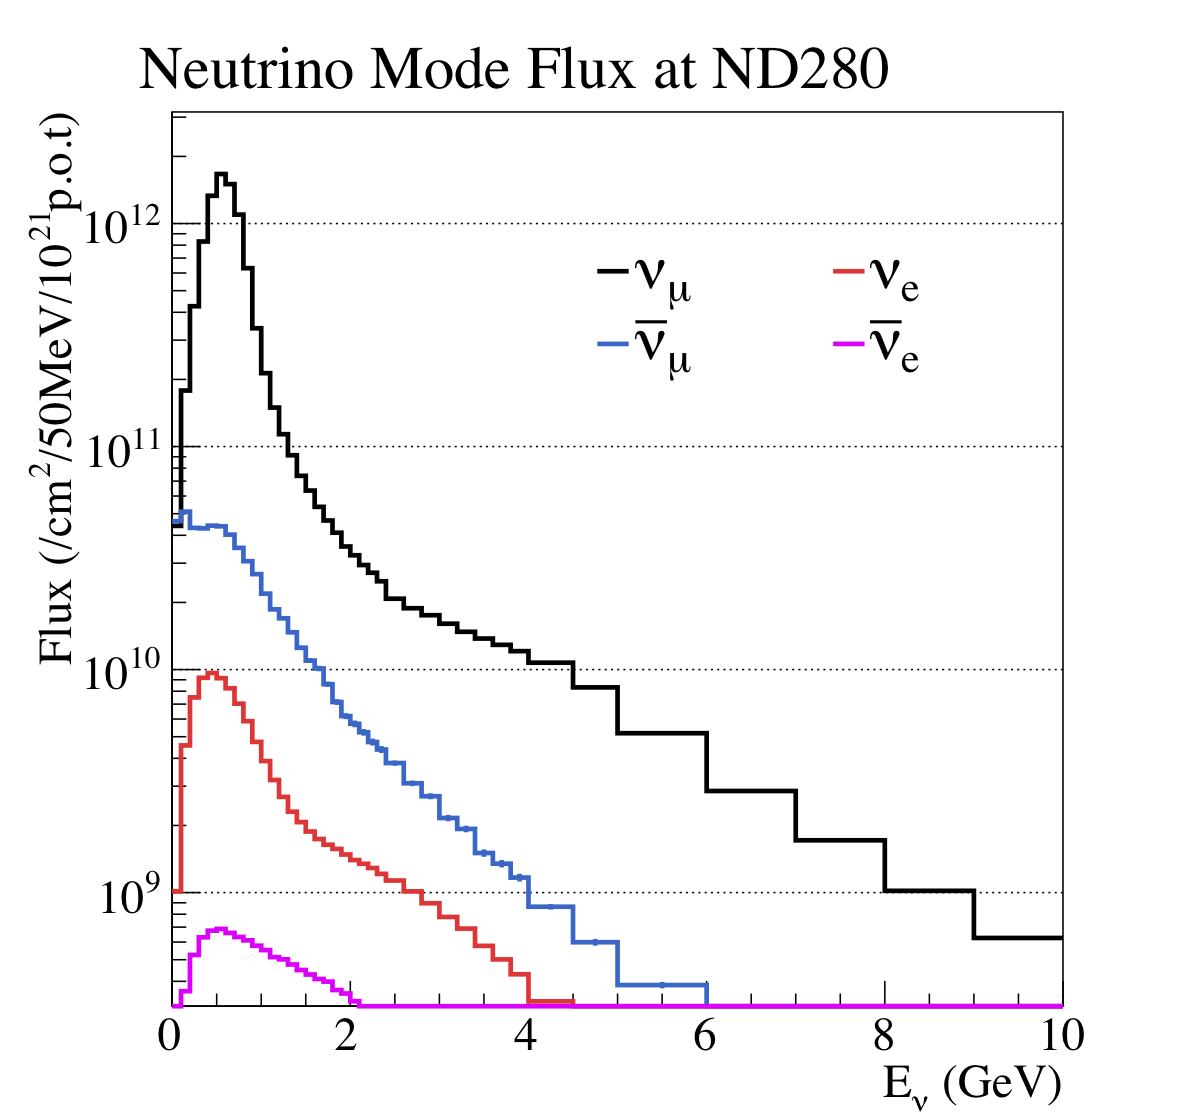
\includegraphics[width=.9\linewidth]{figs/nd5_alltunedflux_run1-9a_zoomed_13a}
  \caption{FHC Mode.}
  \label{fig:fhcmode}
\end{subfigure}%
\begin{subfigure}{.5\textwidth}
  \centering
  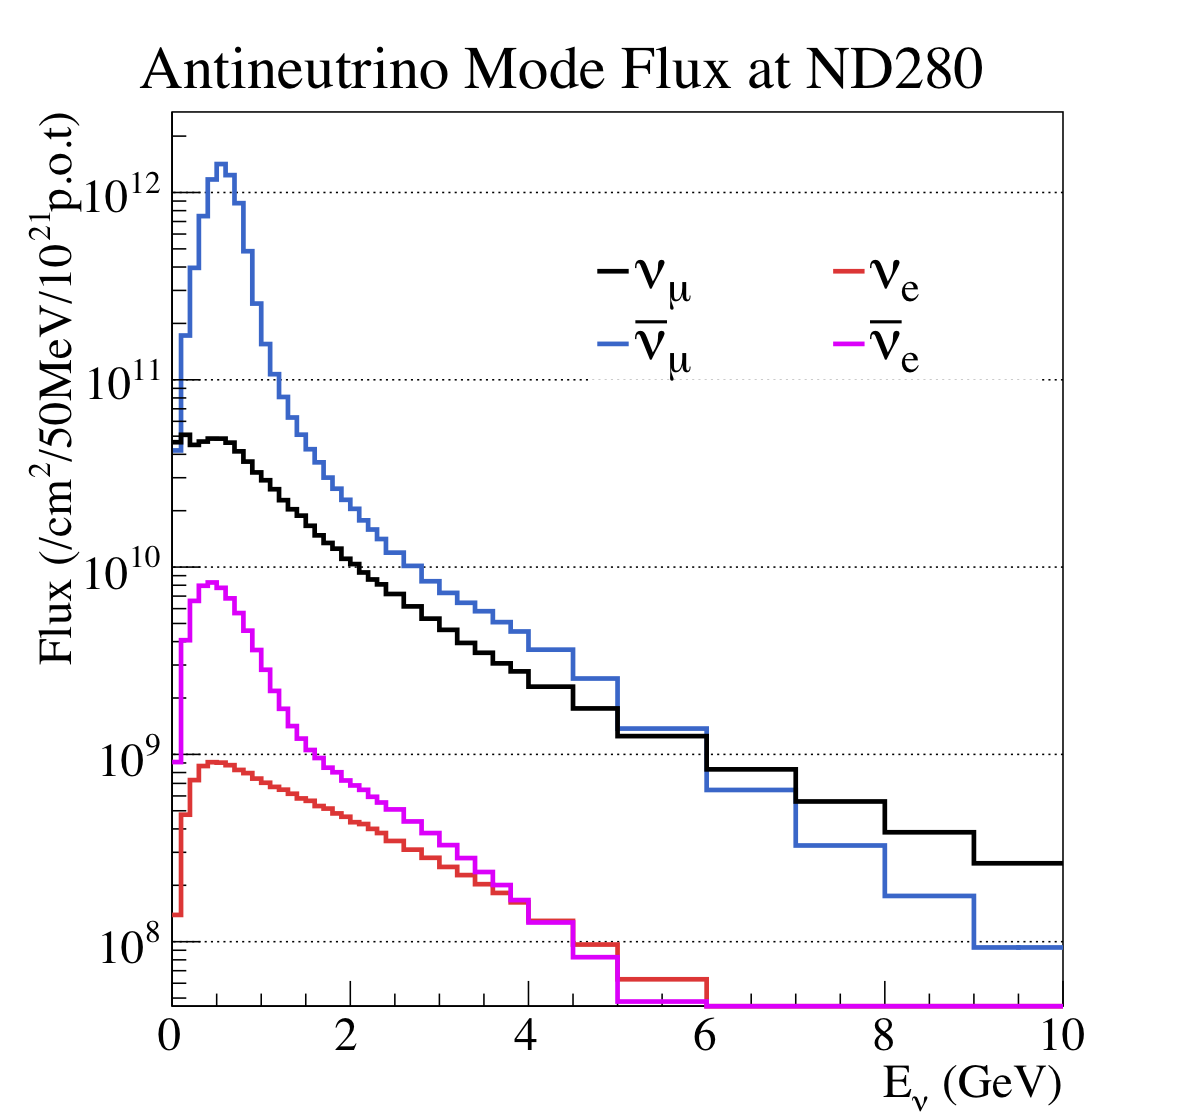
\includegraphics[width=.9\linewidth]{figs/nd5_alltunedflux_run5c-9c_zoomed_antinu_13a}
  \caption{RHC Mode.}
  \label{fig:rhcmode}
\end{subfigure}
\caption{Prediction of ND280 event rate broken down by neutrino species.}
\label{fig:modebreakdown}
\end{figure}

After the decay channel, there is a beam dump made up of 3.17 m of graphite and 2.4 m of iron. This stops all surviving mesons, and all muons below 5 GeV. Neutrinos and higher momentum muons reach the muon monitor (MUMON) beyond the beam dump. The MUMON consists of two independent detectors: Si PIN photodiodes, and ion chambers. These measure the muon profile on a bunch by bunch basis, which is a reliable measure of the beam direction and intensity as the majority of neutrinos in the beam are produced with a muon in a two-body decay. The MUMON measures the beam direction to an accuracy of 0.25 mrad, and the beam intensity to a precision of 3$\%$\cite{mumon}.

It's not possible to count the total number of neutrinos produced in the beam, so the number of protons impinged on the target (POT) is used as a metric for the data collected by T2K. The total accumulated POT and beam power have been increasing since data taking began in 2010, as shown in Figure \ref{fig:pot}. Data from runs 2-9 are used in this analysis.

\begin{figure}[!htbp]
\centering
\includegraphics*[width=0.8\textwidth,clip]{figs/pot}
\caption{The total accumulated POT and beam power at T2K for runs 2-9.} \label{fig:pot}
\end{figure}

\subsection{Off Axis Technique}

Because neutrinos are produced in a two-body decay, and so some fraction of energy is taken by the second decay product, it is not possible to produce a mono-energetic beam. The oscillation probability depends on the neutrino energy, and so more accurate measurements of oscillation parameters can be made using a neutrino beam with a narrower spread of energies. The neutrino energy is given by\cite{Enuoffaxis}:

\begin{equation}
E_{\nu} = \frac{m^{2}_{\pi} - m^{2}_{\mu}}{2(E_{\pi} - p_{\pi} cos\theta_{\pi\nu})}.
\end{equation}

Figure \ref{offaxisEdep} shows $E_\nu$ as a function of $E_\pi$ for different values of $\theta_{\pi\nu}$. The $E_\nu$ distribution is flatter for larger $\theta_{\pi\nu}$, and so $E_\nu$ has a weaker dependence on $E_\pi$. At higher angles a narrower range of $E_\nu$ can therefore be produced from a wider range of $E_\pi$. This effect is highlighted in Figure \ref{offaxis}, showing the predicted neutrino fluxes on and off-axis. A narrower beam spread is produced at 2.5$^o$, but with a lower overall rate (the y-axis is normalised). The beam energy and off-axis angle are chosen such that the neutrino energy peaks at $\sim$0.6 GeV, to maximise the probability of oscillation at the far detector by aligning the beam peak with the first oscillation dip. Going off-axis also reduces the wrong sign contamination in the beam. 

\begin{figure}[!htbp]
\centering
\includegraphics*[width=0.76\textwidth,clip]{figs/offAxisEnergyDep}
\caption{Energy of neutrinos produced in two-body decay as a function of pion energy, for a variety of different off-axis angles.} \label{offaxisEdep}
\end{figure}

\begin{figure}[!htbp]
\centering
\includegraphics*[width=0.6\textwidth,clip]{figs/oaeffect_pnue_pnumu_flux}
\caption{Effect of off-axis angle on the predicted neutrino flux, normalised to arbitrary units, along with the oscillation and survival probabilities of $\nu_{e}$ and $\nu_{\mu}$ respectively.} \label{offaxis}
\end{figure}

\subsection{The Neutrino Flux Simulation}\label{sec:fluxsim}

A data-driven Monte-Carlo (MC) is produced to model the neutrino flux. The FLUKA2008\cite{fluka} software package was used to simulate 30 GeV proton interactions within the target. Measurements from the NA61/SHINE\cite{na61} experiment, which measures interactions of 30 GeV protons in a replica of the T2K target, are used to tune the simulation. The components of the beamline are modelled with the GEANT-4\cite{geant4} based JNUBEAM\cite{jnubeam} software, and secondary interactions and interactions between particles which exit the target with the surrounding area are simulated with the GCALOR package\cite{gcalor}. Secondary particles are tracked until they decay to neutrinos, fall below the energy threshold to decay to neutrinos, or are absorbed in the beam dump. The predicted neutrino energy distributions for FHC mode are shown in Figure \ref{fig:modebreakdown}.

\section{Near Detectors}\label{sec:nd}

The beam is first measured by two near detectors, ND280 and INGRID, 280 m away from the source. At this short distance, the probability of oscillation is negligible and so the unoscillated beam can be measured. The locations of the two detectors within the near detector suite are shown in Figure \ref{ndpit}.

\begin{figure}[!htbp]
\centering
\includegraphics*[width=0.6\textwidth,clip]{figs/ndpit}
\caption{The T2K near detector suite, 280 m from the beam soure. } \label{ndpit}
\end{figure}

\subsection{INGRID}\label{sec:ingrid}

The INGRID detector is located on the beam axis, and is designed to measure the beam profile and direction. From this, the beam angle at ND280 and SK can be determined to within 0.2 mrad, and the beam center to within 5 cm. Neutrino event rates are also measured to within 2$\%$. These measurements are in good agreement with results from MUMON, as shown in Figure \ref{mumoningrid}. A precise determination of the beam direction is necessary as a 1 mrad uncertainty corresponds to a 2-3$\%$ uncertainty on the beam energy.

\begin{figure}[!htbp]
\centering
\includegraphics*[width=0.8\textwidth,clip]{figs/mumoningrid}
\caption{INGRID and MUMON measurements of the beam direction and event rate for runs 1-9.} \label{mumoningrid}
\end{figure}

INGRID achieves this precision by using 16 identical modules made of interleaved iron and scintillator. These are arranged in a 10 x 10 m cross shape centered on the primary proton beamline axis, with 2 modules off-axis outside the cross, as shown in Figure \ref{ingridcross}. 

\begin{figure}[!htbp]
\centering
\includegraphics*[width=0.6\textwidth,clip]{figs/ingridcross}
\caption{The horizontal, vertical, and off-axis modules of the INGRID detector.} \label{ingridcross}
\end{figure}

Each module consists of nine iron sheets and 11 tracking scintillator planes, as shown in Fiugre \ref{ingridmodule}. Each scintillator plane contains 24 horizontal and 24 vertical bars of plastic scintillator. These bars are threaded with a wavelength shifting (WLS) fibre, which collects photons emitted in the plastic scintillator during energy deposition. The WLS fibres transport photons to multi-pixel photon counters (MPPCs) at the end of each bar, and shift the spectrum of the light to the optimal region for MPPC readout. The MPPCs are avalanche photodiodes with a gain 1 x 10$^6$, which convert photons into an electrical signal. This signal is readout by a set of Trip-T front-end electronics boards\cite{tript}, each of which is connected to 48 MPPCs. The backend electronics are made up of readout merger modules (RMM), which read data from the detector, and clock modules, which send trigger signals and ensure all components of the detector are synchronised.

\begin{figure}[!htbp]
\centering
\includegraphics*[width=0.8\textwidth,clip]{figs/ingridmodule}
\caption{The composition of an INGRID module.} \label{ingridmodule}
\end{figure}

The layered structure of each module is surrounded by scintillator planes to veto interactions occurring outside the fiducial volume. The total fiducial mass of iron in each module is 7.1 t, sufficient such that at nominal beam intensity, there are enough neutrino events to measure the beam direction on a day-by-day basis. 

There is another 17th module, with a slightly different composition to the others. This module, known as the proton module, consists of only scintillator planes, but in smaller bars to give a finer granularity. It is designed to detect muons and protons from CCQE interactions on carbon in the plastic, to improve the MC simulation of the beamline and neutrino interactions. The proton module is located at the center of the cross, and like the other modules, is surrounded by veto planes. Figure \ref{protonmodule} shows its composition.

\begin{figure}[!htbp]
\centering
\includegraphics*[width=0.6\textwidth,clip]{figs/protonmodule}
\caption{The composition of the proton module in the INGRID detector.} \label{protonmodule}
\end{figure}

\subsection{ND280}\label{sec:nd280}

The off-axis near detector, ND280, is designed to detect particles produced in neutrino interactions, to determine the event rate of various interaction modes and measure the unoscillated flux and energy of the beam in the direction of SK. This constrains systematic uncertainties allowing more accurate prediction of the event rates at the far detector. ND280 also measures neutrino interaction cross-sections at the 1 GeV energy scale. 

As shown in Figure \ref{nd280basket}, ND280 consists of several sub-detectors. The tracker region contains two time projection chambers (TPCs) between three fine grained detectors (FGDs). The FGDs provide a target for neutrinos, and track particles close to the interaction vertex. The TPCs identify and measure the momentum of particles, particularly muons, which are produced in the event and leave the FGD the interaction vertex is in. The FGDs and TPCs are described in more detail in Sections \ref{sec:fgd} and \ref{sec:tpc}.

\begin{figure}[!htbp]
\centering
\includegraphics*[width=0.6\textwidth,clip]{figs/nd280basket}
\caption{Exploded view of ND280, showing it's sub-detectors.} \label{nd280basket}
\end{figure}

Upstream of the tracker, the $\pi^0$ detector (P0D) detects NC events on water, the same target as in the far detector. This is described in Section \ref{sec:pod}. Both the tracker region and P0D are surrounded by electromagnetic calorimeters (ECals). The ECals are designed to measure the energy of photons produced in the inner detectors and reconstruct $\pi^0$ tracks from the FGDs. They are described in more detail in Section \ref{sec:ecal}.

The whole detector sits within the UA1 magnet which produces a 0.2 T magnetic field. This allows accurate charge and momentum measurements in the TPCs. The magnet yoke is interleaved with scintillator, the side muon range detector (SMRD). This measures high angle muons exiting the detector, cosmic ray muons entering the detector, and interactions in the magnet and surrounding area. The magnet and SMRD are described in Section \ref{sec:mag}.

The same MPPCs used in INGRID are also used throughout ND280. These were chosen, rather than the more common photomultiplier tubes (PMTs), as they can be used within a magnetic field. 

\subsubsection{The Fine Grained Detectors}\label{sec:fgd}

The FGDs provide the primary target for neutrino interactions in ND280. They are designed to be able to measure particles which don't exit themselves and enter a TPC. To achieve this, they are completely active, allowing them to measure vertex activity and short range tracks such as those from recoil protons. Short ranged particles tend to have low momentum and deposit lots of energy per track length, and so the FGDs need to be able to detect charged particles with fine granular resolution, to distinguish between tracks and determine their direction. 

The FGDs are also used as a cosmic trigger for stopping pions, which allows the identification and reconstruction of subsequent Michel electrons. They are also used for measurements of the time-of-flight (TOF) of tracks to differentiate between forward-going positive and backward-going negative particles. As well as this, the FGDs have the best timing resolution of all the sub-detectors, and are used as the base for reconstructing tracks which pass through more than one sub-detector. 

The two FGDs both contain 1.1 t of target mass, and consist of layers of scintillator bars. Each layer is 186.4 x 186.4 x 2.02 cm, and contains 192 bars in the horizontal direction and 192 bars in the vertical direction. The bars are covered in a reflective coating containing TiO$_2$, and each are 96 x 96 x 186.4 cm. A WLS fibre runs down the centre of each bar to an MPPC at the end. The other end is mirrored by a vacuum deposition of aluminium.

The most upstream FGD (FGD1) is composed of 15 scintillator planes. The second FGD (FGD2) has 7 scintillator planes separated by layers of hollow corrugated polycarbonate sheets. These are filled with water, providing a water-scintillator hybrid target. The FGDs therefore measure interactions on CH in the scintillator, which is a common target in external neutrino scattering experiments, and H$_2$O, the far detector target. Nuclear effects cannot be accurately extrapolated between target nuclei, and so it useful to be able measure interaction rates on water at ND280.

The resolution and track length in the FGDs is too low to use d$E$/d$x$ to identify particles which don't enter the TPCs, so the combination of integrated deposited energy and track length is used. These quantities are compared to theoretical values for different particles, as shown in Figure \ref{fig:FGD1}, allowing protons to be distinguished from other charged particles. In particular, accurately distinguishing protons and pions which stop in the FGDs is vital for correctly identifying the interaction type. Figure \ref{fig:FGD1} shows data from both the neutrino beam, and cosmic trigger. The neutrino beam data contains particles identifiable as protons, muons, and pions, whereas the cosmic trigger data only contains particles identifiable as muons and pions, as would be expected.

\begin{figure}
\centering
\begin{subfigure}{.5\textwidth}
  \centering
  \includegraphics[width=0.95\linewidth]{figs/FGD1beam}
  \caption{Neutrino beam data.}
  \label{fig:fgd1beam}
\end{subfigure}%
\begin{subfigure}{.5\textwidth}
  \centering
  \includegraphics[width=0.95\linewidth]{figs/FGD1cosmic}
  \caption{Cosmic trigger data.}
  \label{fig:FGD1cosmic}
\end{subfigure}
\caption{Integrated deposited energy as a function of range for particles stopping in FGD1. The scatter plot shows data while the curves show the MC predictions for protons, muons, and pions.}
\label{fig:FGD1}
\end{figure}

\subsubsection{The Time Projection Chambers}\label{sec:tpc}

The three TPCs are located either side of each FGD, and provide high resolution tracking for both forward-going and backward-going particles. The majority of the particle identification and momentum measurements at ND280 take place inside them. The multiplicity and direction of tracks can be easily determined, as the TPCs detect events in 3 dimensions. The momentum of particles can be measured from the bending of tracks in the TPCs due to the magnetic field.

The construction of the three TPCs is identical. They consist of two concentric boxes, as shown in Figure \ref{fig:tpcconstruction}. The inner box is filled with a drift gas consisting of an Ar:CF$_4$:C$_4$H$_{10}$ mixture at 95:3:2. The walls of the inner box form the field cage. The outer box walls are held at ground voltage, and the outer box is filled with CO$_2$, to provide electrical insulation between the boxes. 

\begin{figure}[!htbp]
\centering
\includegraphics*[width=0.6\textwidth,clip]{figs/tpc}
\caption{Schematic diagram of a TPC module.} \label{fig:tpcconstruction}
\end{figure}

The inner box contains the cathode, and the walls parallel to the cathode have a copper pattern, designed to produce a uniform electric field in the module aligned with the magnetic field. The TPC modules are made of non-magnetic materials as not to interfere with the field from the magnet. 

When a charged particle passes through a TPC module, ionisation electrons are produced, which drift away from the cathode to readout planes on the walls of the inner box. Here, the electrons are multiplied and detected by micromegas detectors. The time and position of the electron signals at the readout planes give a 3D image of the particle track.

Particle identification is performed in the TPCs using, like in the FGDs, d$E$/d$x$. This is shown in Figure \ref{fig:tpcpid}, as a function of momentum, for different particles. The d$E$/d$x$ resolution is 7.8$\pm$0.2$\%$, allowing electrons and muons to be distinguished. 

\begin{figure}[!htbp]
\centering
\includegraphics*[width=0.6\textwidth,clip]{figs/tpcpid}
\caption{Energy loss as a function of momentum for particles in one TPC. The scatter plot shows data while the curves show the MC predictions for protons, electrons, muons, and pions.} \label{fig:tpcpid}
\end{figure}


\subsubsection{The $\pi^0$ Detector}\label{sec:pod}

The P0D was designed to measure the cross-section of the neutral current interaction $\nu_\mu + N \rightarrow \nu_\mu + N + \pi^0 + X$ on water. This is one of the major backgrounds to $\nu_e$ appearance at the far detector, and so it is necessary to measure and constrain it.

The P0D is located upstream of the FGDs and TPCs. It consists of alternating layers of scintillator bars, brass and lead sheets, and water target bags, as shown in Figure \ref{fig:podconstruction}. There are 40 modules, each made up of two triangular scintillator bars. The first layer contains 134 vertical bars, and the second 126 horizontal bars. Each bar contains a WLS fibre which is read out by an MPPC. The horizontal and vertical bars are 234 and 220 cm long respectively.

\begin{figure}[!htbp]
\centering
\includegraphics*[width=0.6\textwidth,clip]{figs/podconstruction}
\caption{A schematic diagram of the side on view of the P0D.}\label{fig:podconstruction}
\end{figure}

The water bags can be emptied, allowing measurements of the cross-section on H$_2$O by subtraction. The target mass is 16.1 t with water in the bags, and 13.3 t without water. The lead and brass sheets produce electron showers which can be detected, from photons emitted in $\pi^0$ decays.

\subsubsection{The Electromagnetic Calorimeter}\label{sec:ecal}

The primary purpose of the ECals is to tag and reconstruct $\pi^0$s from the FGD, TPC, and P0D, by measuring the energy and direction of photon showers. It is also used to distinguish between pions and muons by shower shape. The ECal's near hermetic coverage of the inner detectors allows full reconstruction of events, and they also provide complimentary particle identification to the TPCs.

There are three sections of the ECal: the downstream ECal (DsECal) located after the last TPC, the barrel ECal surrounding the FGDs and TPCs, and the P0D ECal surrounding the P0D. These are shown in Figure \ref{nd280basket}. The barrel and downstream ECals are tracking calorimeters which reconstruct electromagentic showers, particularly those from high-angle particles from the TPC. The P0D ECal is designed to tag energy escaping from the P0D and distinguish photons from muons, as the P0D reconstructs showers itself.

Each ECal module consists of alternating layers of scintillator bars and lead sheets. The bars are 40 x 10 mm, and contain a WLS fibre which is read out by an MPPC. The lead sheets are 1.75 mm thick.

The downstream ECal has 34 layers of scintillator, corresponding to 11 electron radiation lengths. Alternate layers are orientated perpendicularly to each other. This gives two `views', which can be combined to create 3D reconstructed tracks. The downstream ECal is 2300 x 2300 x 500 mm, and its total target mass is 4.80 t.

The 6 modules of the barrel ECal have 31 layers of scintillator, corresponding to 10 electron radiation lengths. These also alternate orientations similarly to the downstream ECal. The side barrel ECal modules are 4140 x 2500 x 462 mm, and their total target masses are 9.21 t. The top and bottom barrel ECals are 4140 x 1676 x 462 mm, and their total target masses are 6.62 t.

The 6 modules of the P0D ECal have only 6 layers of scintillator, each parallel to the beam. These are interspersed with 4 mm thick lead sheets. The side P0D ECal modules are 2898 x 2454 x 155 mm, and their target masses are 2.64 t. The top and bottom P0D ECal modules are 1584 x 2454 x 155 mm, and their target masses are 1.5 t.

\subsubsection{The UA1 Magnet and Side Muon Range Detector}\label{sec:mag}

The TPC, FGD, P0D, and ECal all sit within the UA1 magnet, which provides a 0.2 T magnetic field. This allows the TPCs to measure the momentum of charged particles with a resolution of 10$\%$, and determine their sign, which identifies if the interaction involved a neutrino or anti-neutrino. The magnet consists of water-cooled aluminium coils, which produce the field. The coils are supported by the return yoke, which is made up of 16 C-shaped iron elements. The internal volume of the magnet is 7.0 x 3.5 x 3.6 m, and the external volume is 7.6 x 5.6 x 6.1 m.

The nominal current is 2.7 kA, and this is monitored regularly to accurately calculate the field. This reduces the uncertainty on momentum measurements in the TPC. The uncertainty on the field measurement is 2 x 10$^{-4}$ T.

Air gaps in the return yoke hold the modules of the SMRD. These are used to track high angle muons and measure their momentum, as well as providing a cosmic trigger. The SMRD consists of 192 horizontal and 248 vertical plastic scintillator modules. The horizontal modules are 9 × 686 × 955 mm, and the vertical modules are 9 × 892 × 955 mm. The scintillator modules contain a WLS fibre which is read out by an MPPC.

\subsubsection{The Data Acquisition System}\label{sec:daq}

The ND280 data acquisition (DAQ) system triggers the readout of information from each of the sub-detectors, as well as the storage of recorded data. The same system is used for both ND280 and INGRID.

There are three trigger requirements during physics runs: the beam trigger, when a beam spill occurs; the Trip-T cosmic trigger, when hits are seen on the opposite sides of the outer detectors (top and bottom SMRD, left and right SMRD, or P0D and downstream ECal) outside the beam window; and the FGD cosmic trigger, when hits are seen in both FGDs outside the beam window. These initiate a fixed time window during which data is recorded. Data is acquired from front-end electronic boards via optical Gigabit links, and event fragments from the sub-detectors are merged and logged.

\subsection{Near Detector Simulation}\label{sec:ndsim}

The ND280 and INGRID geometries and the paths of final-state particles from neutrino interactions are simulated in GEANT-4. The neutrino interactions themselves are simulated using NEUT \cite{neut}, an interaction generator written for the Super-Kamiokande and T2K experiments.

A custom software package, ElecSim, is used to simulate the response of the detector and electronics to energy deposited by particles that have propagated through the detectors. This involves simulating the light emitted from the energy deposition, the transport of that light through the bar and down the WLS fibres, and the subsequent response of the MPPCs. For the TPCs, ElecSim simulates the electron drift and response of the micromegas detectors. 

\section{Super-Kamiokande}\label{sec:SK}

The far detector, Super-Kamiokande, is a water Cherenkov detector located 295 km west of the near detector suite, in the Kamioka mine inside Mt. Ikenoyama. The mine provides 1 km of rock (or 2.7 km equivalent of water), shielding the detector from cosmic ray muons below 1.3 TeV, significantly reducing background rates. The detector is filled with 50 kt of pure water (25 kt fiducial volume), and, like ND280, lies 2.5$^o$ off-axis. Figure \ref{fig:superk} shows the detector within the mine.

\begin{figure}[!htbp]
\centering
\includegraphics*[width=0.6\textwidth,clip]{figs/Superk}
\caption{The Super-Kamiokande detector within the Kamioka mine.}\label{fig:superk}
\end{figure}

Super-Kamiokande has been searching for proton decay and measuring solar and atmospheric neutrino oscillations since 1996, and has been a far detector for a long baseline accelerator neutrino oscillation experiment since 1999, initially for K2K and now for T2K. Although it has undergone several updates during this period, the long running operation mean its behaviour is well understood. The atmospheric and cosmic ray muon data provide calibration samples completely separate from the T2K analysis, for which the simulated MC matches data to the percent level.

The detector is divided into the inner (ID) and outer (OD) detectors by a 55 cm cylindrical stainless steel and tyvek framework. The OD is 40.2 m in height with a radius of 35.8 m. It surrounds the ID with 2 m of water, serving as a shield from interactions in the surrounding rock. 1885 outward-facing 20 cm PMTs provide an active veto for cosmic ray muons with an efficiency of almost 100$\%$, despite the fairly sparse PMT coverage. The beam timing window can be used to identify interactions in the OD from beam neutrinos.

The ID is 36.2 m in height with a radius of 33.8 m. It contains 11,129 inward-facing 50 cm PMTs, each with a combined quantum and collection efficiency of 20$\%$, and a timing resolution of $\sim$2 ns. The PMT coverage of the ID is 40$\%$, which gives enough spatial resolution to sufficiently reconstruct the paths of particles produced in neutrino interactions inside the tank.

When charged particles travel through a medium of refractive index $n$ at a velocity $v_p$ larger than the speed of light in the medium, $v_\gamma = c/n$, Cherenkov radiation is emitted in a cone with opening angle $\theta_c$ = arcos$\frac{1}{n\cdot v/c}$, along the direction of the particle's path. In water, this is $\sim$42$^o$. Neutrino interactions in the SK tank produce charged particles which, if above an energy threshold, can be detected by the emitted Cherenkov light. Photons from the cone form a ring shape on the walls of the tank, where they are detected by the PMTs. This pattern, along with the hit timing, can be used to reconstruct the interaction vertex position, and the charge, momentum and direction of the produced particle.

CCQE interactions are the primary channels used to measure $\nu_\mu$ disappearance and $\nu_e$ appearance at T2K. Discounting final state interactions, these events produce a charged lepton and a proton. The measured momentum and direction of the lepton can be used to reconstruct the neutrino energy, using Equation \ref{eqn:erec}, but it is also vital for the lepton flavour to be determined, as this corresponds to the incoming neutrino flavour.

Discrimination between electrons and muons is achieved by separating Cherenkov rings by shape. As electrons are relatively light, they scatter off particles in the water and so travel a more convoluted path to the PMTs. At the T2K beam energies, they will also induce electromagnetic showers. Both of these phenomena cause the Cherenkov light to form a superposition of overlapping rings at the wall of the ID. This results in a fuzzy ring being seen in the PMTs.

Conversely muons, due to their relatively large mass, travel through the water without scattering, and so produce a sharp, clear Cherenkov ring. Examples of electron and muon Cherenkov rings detected at SK are shown in Figure \ref{fig:skeventdisplay}.

\begin{figure}
\centering
\begin{subfigure}{.5\textwidth}
  \centering
  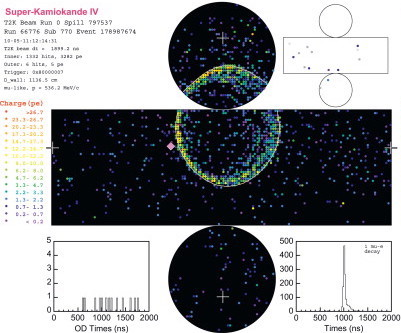
\includegraphics[width=0.95\linewidth]{figs/skeventdisplayelectron}
  \caption{Muon neutrino event.}
  \label{fig:skeventdisplayelectron}
\end{subfigure}%
\begin{subfigure}{.5\textwidth}
  \centering
  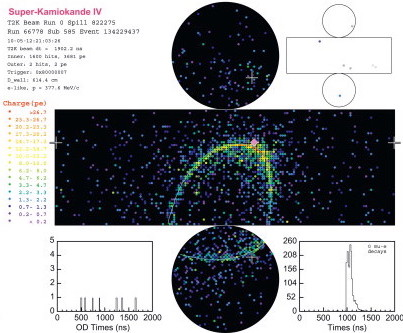
\includegraphics[width=0.95\linewidth]{figs/skeventdisplaymuon}
  \caption{Electron neutrino event.}
  \label{fig:skeventdisplaymuon}
\end{subfigure}
\caption{SK ID event display, showing the Cherenkov ring PMT hits for an a) electron, and b) muon neutrino event. }
\label{fig:skeventdisplay}
\end{figure}

An algorithm\cite{skrecoalg} is used to distinguish between fuzzy and sharp rings with high efficiency. The probability of a muon neutrino event being misidentified as an electron neutrino event is 0.7$\%$. The number of different neutrino species events is used to calculate neutrino oscillation parameters in the full T2K oscillation analysis. However, as Super-Kamiokande does not have a magnetic field, it is not able to differentiate between neutrino and anti-neutrino interactions. The neutrino and anti-neutrino content of the beam is therefore needed to be measured accurately at ND280. In this analysis, only data from ND280 is used, to constrain systematic uncertainties.

\subsection{Far Detector Simulation}

Neutrino interactions in the SK tank are modelled by the NEUT event generator. The simulation of produced particles through the detector is done using the GEANT-3\cite{geant3} based SKDETSIM software. Like in the beam production, hadronic interactions are simulated with the GCALOR package.

\newpage